\documentclass[11pt]{article}
\usepackage[T1]{fontenc}
\usepackage[utf8]{inputenc}
\DeclareUnicodeCharacter{00A0}{~}
\usepackage{lmodern}
\usepackage[ngerman]{babel}
\usepackage{microtype}

\usepackage{graphicx}
\usepackage[hypertexnames=false]{hyperref}
\usepackage{xurl}
\usepackage{xcolor}
\usepackage{pdflscape}

\usepackage{tikz}
\usetikzlibrary{arrows.meta,positioning}
\usetikzlibrary{calc,chains,shapes,fit}

\graphicspath{{diagrams/}}
\usepackage{float}

\usepackage{array}
\usepackage{ragged2e}
\usepackage{tabularx}
\usepackage{longtable}
\usepackage{ltablex}
\keepXColumns

\usepackage{listings}

\usepackage{geometry}
\geometry{a4paper, top=20mm, left=20mm, right=20mm, bottom=25mm}

\usepackage{fancyhdr}
\setlength{\headheight}{15pt}
\pagestyle{fancy}
\lhead{Luca Güttinger}
\rhead{\today}
\rfoot{Seite \thepage}
\cfoot{}
\lfoot{\footnotesize\mbox{\url{https://github.com/Notenverwaltung-ch/Notenverwaltung}}}

\lstset{
    inputencoding=utf8,
    language=SQL,
    basicstyle=\small\ttfamily,
    breaklines=true,
    breakatwhitespace=true,
    columns=fullflexible,
    keepspaces=true,
    showstringspaces=false,
    tabsize=2,
    postbreak=\mbox{\textcolor{red}{$\hookrightarrow$}\space},
    literate={ä}{{\"a}}1 {ö}{{\"o}}1 {ü}{{\"u}}1 {Ä}{{\"A}}1 {Ö}{{\"O}}1 {Ü}{{\"U}}1 {ss}{{\ss}}1 {é}{{\'e}}1 {è}{{\`e}}1 {à}{{\`a}}1 {ê}{{\^e}}1 {ô}{{\^o}}1 {É}{{\'E}}1
}

\newcommand{\code}[1]{\texttt{\detokenize{#1}}}

\newcolumntype{L}[1]{>{\raggedright\arraybackslash}p{#1}}
\newcolumntype{C}[1]{>{\centering\arraybackslash}p{#1}}
\newcolumntype{R}[1]{>{\raggedleft\arraybackslash}p{#1}}
\newcolumntype{Y}{>{\raggedright\arraybackslash}X}

\setlength{\parindent}{0pt}
\setlength{\parskip}{6pt}

\setcounter{tocdepth}{4}
\setcounter{secnumdepth}{4}

\begin{document}

    \hypersetup{pageanchor=false}
% ---------------- Titelseite ----------------
    \begin{titlepage}
        \centering
        {\huge\bfseries Notenverwaltungssystem \par}
        \vspace{2cm}
        {\Large Luca Güttinger \par}
        \vspace{0.5cm}
        {\Large Dipl. Informatiker Applikationsentwicklung \par}
        \vspace{0.5cm}
        {\Large TEKO Zürich \par}
        \vspace{0.5cm}
        {\Large Netzwerkbetriebsysteme \par}
        {\Large Dozent: Uta Enke \par}
        \vspace{0.5cm}
        {\Large Abgabedatum: 22.09.2025 \par}
        \vfill
    \end{titlepage}
    \clearpage
    \hypersetup{pageanchor=true}
    \pagenumbering{arabic}

% ---------------- Inhaltsverzeichnis ----------------
    \tableofcontents
    \newpage


    \section{Einleitung}

    \subsection{Ziel}

    \subsection{Voraussetzungen}


    \section{Architektur}

    \subsection{Übersicht}

    % Architekturdiagramm
    \begin{figure}[H]
        \centering
        \resizebox{\linewidth}{!}{
            \begin{tikzpicture}[
                every node/.style={font=\small},
                box/.style={draw, rounded corners, thick, align=center, inner sep=6pt, fill=white, text width=4.6cm},
                group/.style={draw, rounded corners, thick, align=center, inner sep=8pt, fill=gray!10},
                rel/.style={-Latex, thick},
                edgelabel/.style={font=\scriptsize, fill=white, inner sep=1pt, text=black}
            ]
                % Cloudflare DNS
                \node[box, fill=orange!20, minimum width=5.5cm, text width=5.2cm] (cloudflare) {Cloudflare DNS\\DNS Records\\\texttt{A/AAAA} -> Server IP};

                % Hetzner Cloud Server (full width)
                \node[group, below=1.8cm of cloudflare, minimum width=17.0cm, minimum height=1.0cm, anchor=north] (hetzner) {Hetzner Cloud Server};

                % Docker network group inside Hetzner (full width)
                \node[group, below=1.4cm of hetzner.south, anchor=north, minimum width=16.6cm, minimum height=10.4cm] (net) {};

                % Containers inside the Docker network (proxy on top, three services side-by-side)
                % Proxy NGINX (exposed 80) near top center
                \node[box, fill=blue!15, minimum width=5.6cm, text width=5.2cm] (proxy) at ($(net.north)!0.28!(net.south)$) {NGINX Reverse Proxy\\exposed: 80/tcp};

                % T-shape: Spring centered under proxy; Angular left; pgAdmin right with tight spacing
                \node[box, fill=teal!15, below=1.6cm of proxy, minimum width=5.0cm, text width=4.6cm] (spring) {Spring Boot API\\internal: 8080};
                \node[box, fill=green!15, left=0.4cm of spring, minimum width=5.0cm, text width=4.6cm] (angular) {Angular App\\internal: 80};
                \node[box, fill=purple!15, right=0.4cm of spring, minimum width=5.0cm, text width=4.6cm] (pgadmin) {pgAdmin\\internal: default port};

                % External access arrows to proxy (split to avoid overlap)
                \node[edgelabel, above=0.4cm of hetzner.north] (dnshttp) {HTTP 80};
                \node[edgelabel, left=0.0cm of dnshttp, xshift=-2.0cm] (host1) {notenverwaltung.ch};
                \node[edgelabel, right=0.0cm of dnshttp, xshift=2.0cm] (host2) {api.notenverwaltung.ch};
                \node[edgelabel, below=0.0cm of dnshttp] (host3) {pgadmin.notenverwaltung.ch};
                \draw[rel] (cloudflare.south) -- (hetzner.north);
                \draw[rel] (hetzner) -- (proxy);

                % Proxy routing rules: straight down to Spring; short diagonals to Angular/pgAdmin
                \draw[rel] (proxy.south) -- node[edgelabel]{api.notenverwaltung.ch:80} (spring.north);
                \draw[rel] (proxy.south west) -- node[edgelabel, left]{notenverwaltung.ch:80} (angular.north east);
                \draw[rel] (proxy.south east) -- node[edgelabel, right]{pgadmin.notenverwaltung.ch:80} (pgadmin.north west);

                % Centered container group box sized to full width appearance
                \node[draw, rounded corners, thick, minimum width=16.0cm, minimum height=8.8cm, anchor=center] (containersbox) at (net.center) {};
                \node[above=2mm of containersbox.north] {Container im Netzwerk};
                % Docker Network label moved inside the containers box (top-left corner)
                \node[anchor=north west, font=\small, align=left] at ([xshift=3mm,yshift=-3mm]containersbox.north west) {Docker Network: \texttt{notenverwaltung\_productive}};

            \end{tikzpicture}
        }
        \caption{Architekturübersicht: Reverse Proxy, Angular Frontend, Spring API und pgAdmin in Docker-Netzwerk auf Hetzner. DNS via Cloudflare.}
        \label{fig:architecture}
    \end{figure}

    \subsection{Hetzner Cloud Server}
    Es wird ein Cloud Server bei Hetzner verwendet. Der Server hat folgende Spezifikationen:
    \begin{itemize}
        \item Name: CPX21
        \item 4 GB RAM
        \item 80 GB SSD
        \item 20 TB Traffic
        \item Ubuntu 24.04 LTS
        \item 3 vCPUs (AMD EPYC 7002 Series)
        \item 1 IPv4 Adresse
    \end{itemize}

    Zusätzlich wird ein Volume mit 20 GB Speicherplatz hinzugefügt, damit die Daten der Datenbank persistent gespeichert werden.

    \subsection{Cloudflare}


    \section{Deploymment}

    \subsection{Github Actions}

    \subsection{Spring Applikation}

    \subsection{Angular Frontend}


    \section{Installation}

    \subsection{Vorbereitungen}
    Auf den Server wird via SSH zugegriffen. Dazu wird ein SSH Key Paar erstellt und der Public Key auf dem Server hinterlegt.
    In dem Fall passiert mit dem auswählen des SSH Keys in der Hetzner Cloud Console.

    \subsubsection{Volume hinzufügen}
    Damit die Daten der Datenbank persistent gespeichert werden, wird ein Volume erstellt und dem Server hinzugefügt.

    Das Passiert mit folgenden Befehlen:
    \begin{lstlisting}{language=bash}
        mkfs.ext4 -F  /dev/disk/by-id/scsi-0HC_Volume_<voulmeID>
        mkdir /mnt/volume-nbg1-1
        mount -o discard,defaults /dev/disk/by-id/scsi-0HC_Volume_<voulmeID> /mnt/volume-nbg1-1
        echo "/dev/disk/by-id/scsi-0HC_Volume_<voulmeID> /mnt/volume-nbg1-1 ext4 discard,nofail,defaults 0 0" >> /etc/fstab
    \end{lstlisting}

    \subsubsection{Firewall}
    In Hetzner ist eine Firewall konfiguriert, die nur den Zugriff auf die Ports 22 (SSH), 80 (HTTP) und 443 (HTTPS) erlaubt.
    \begin{figure}
        \centering
        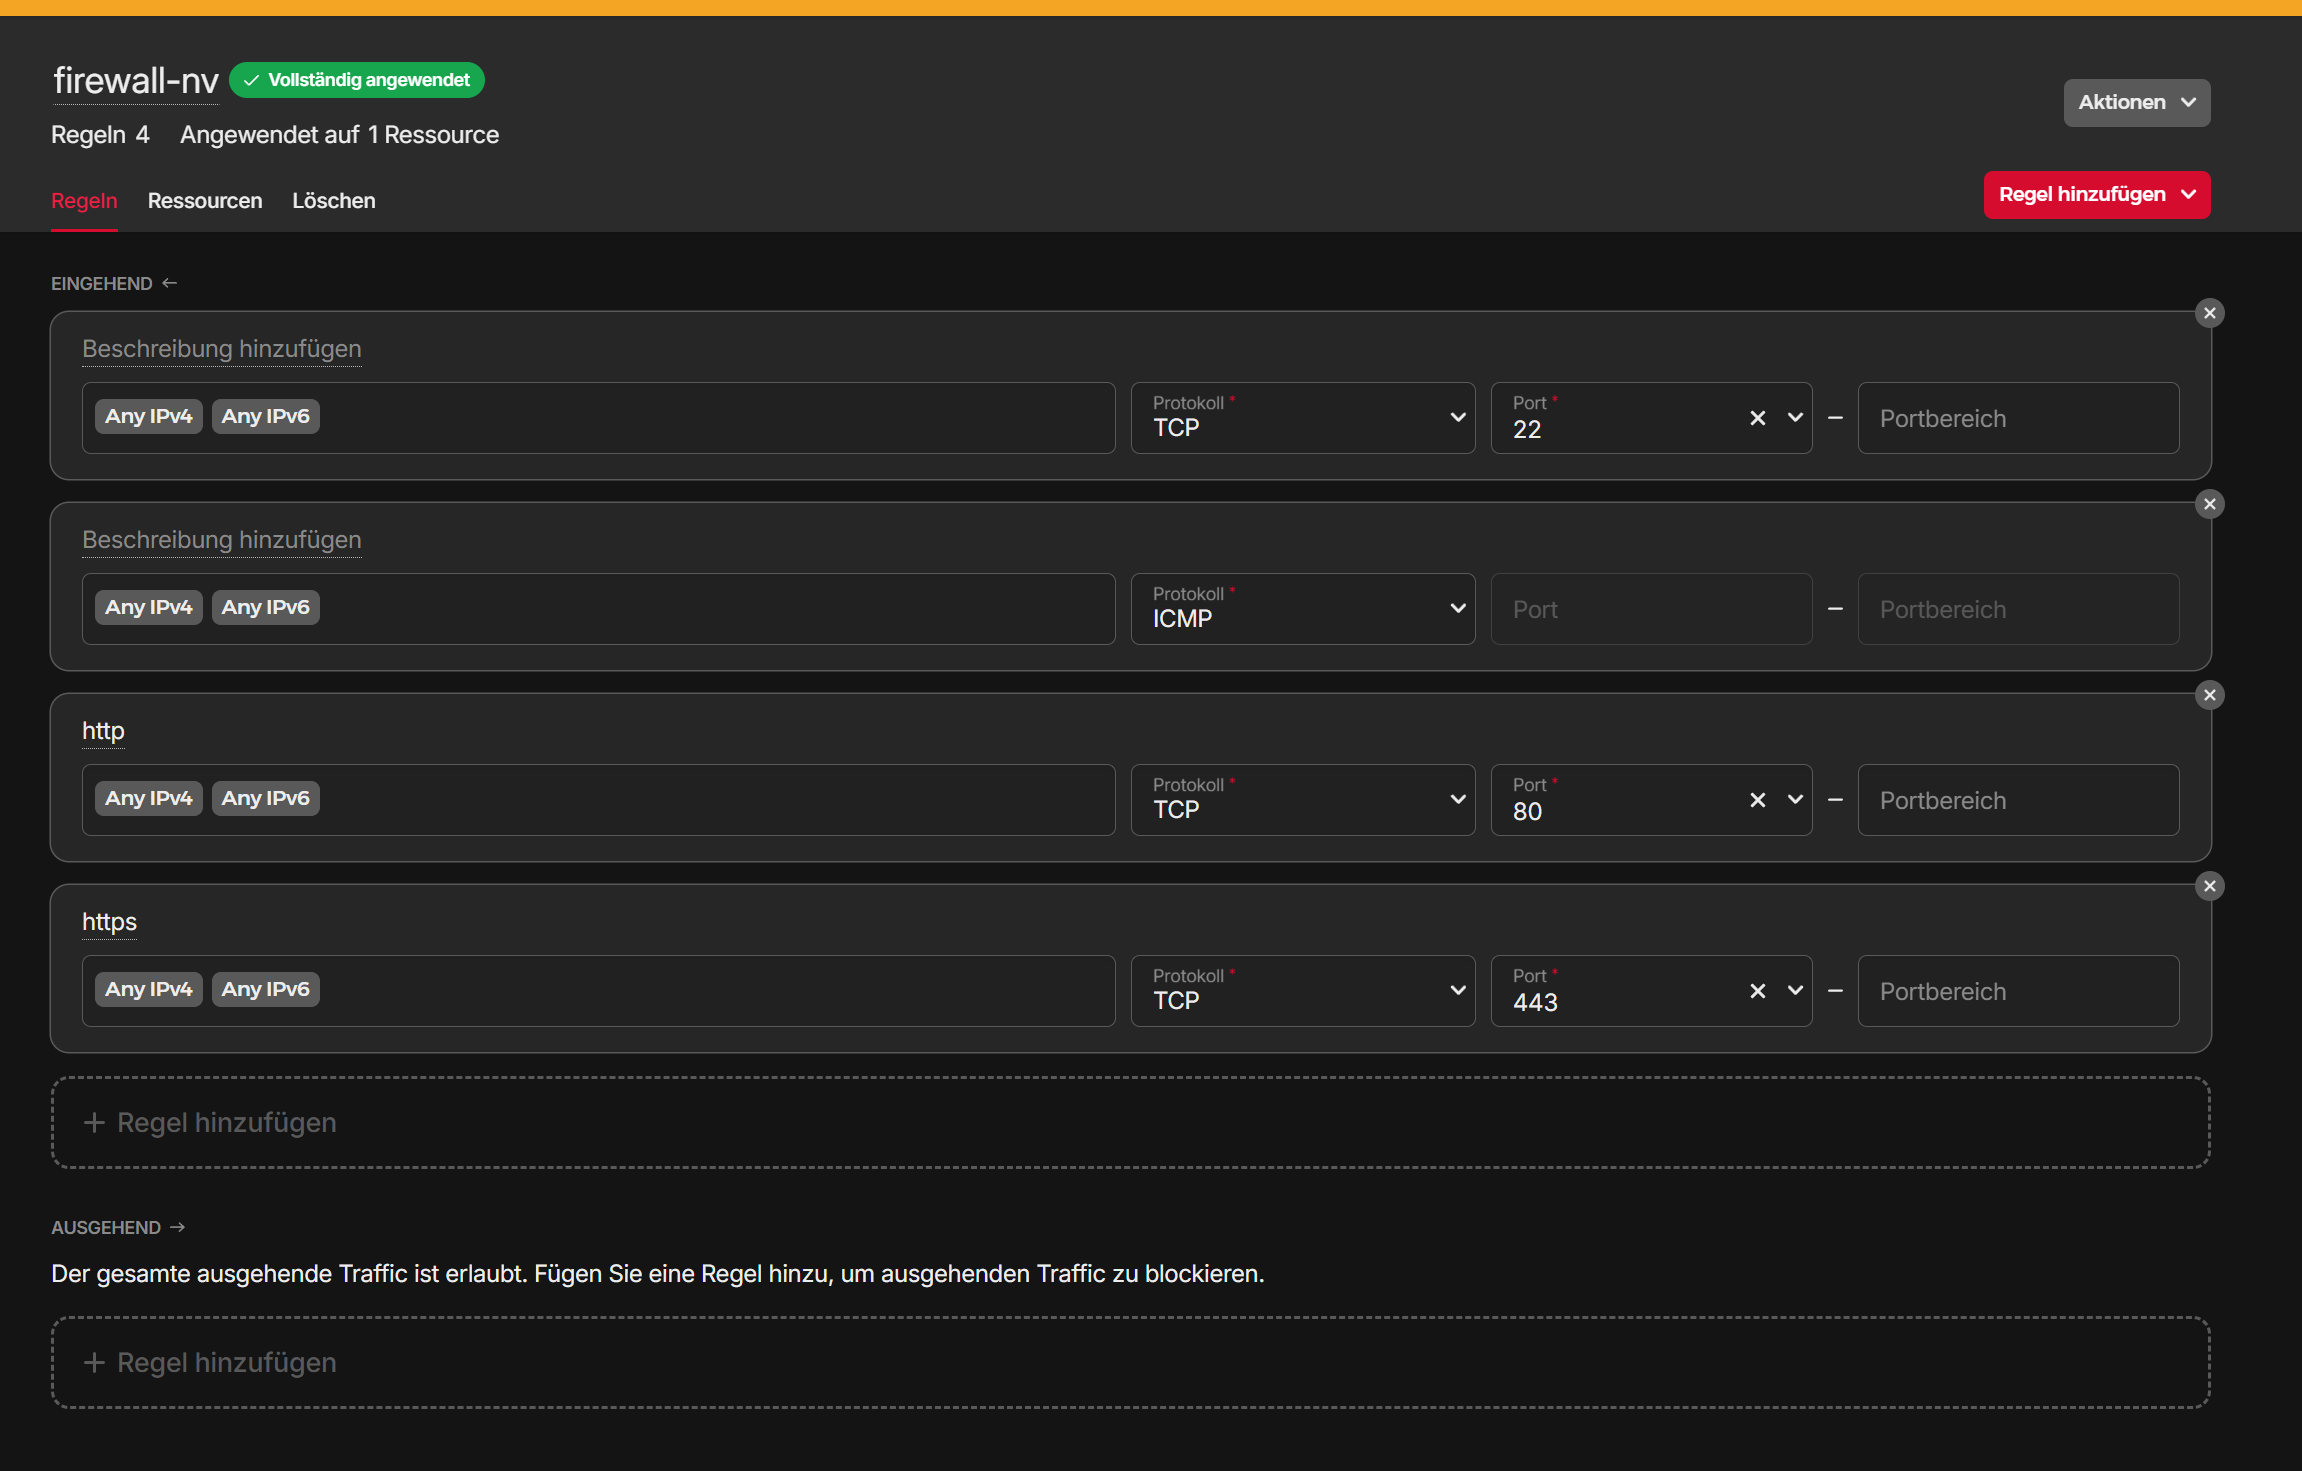
\includegraphics[width=0.95\linewidth]{images/firewall}
        \caption{Firewall in Hetzner}
        \label{fig:firewall}
    \end{figure}

    \subsubsection{DNS}
    In Cloudflare werden die DNS Records erstellt, damit die Domain auf die IP Adresse des Servers zeigt.
    \begin{figure}
        \centering
        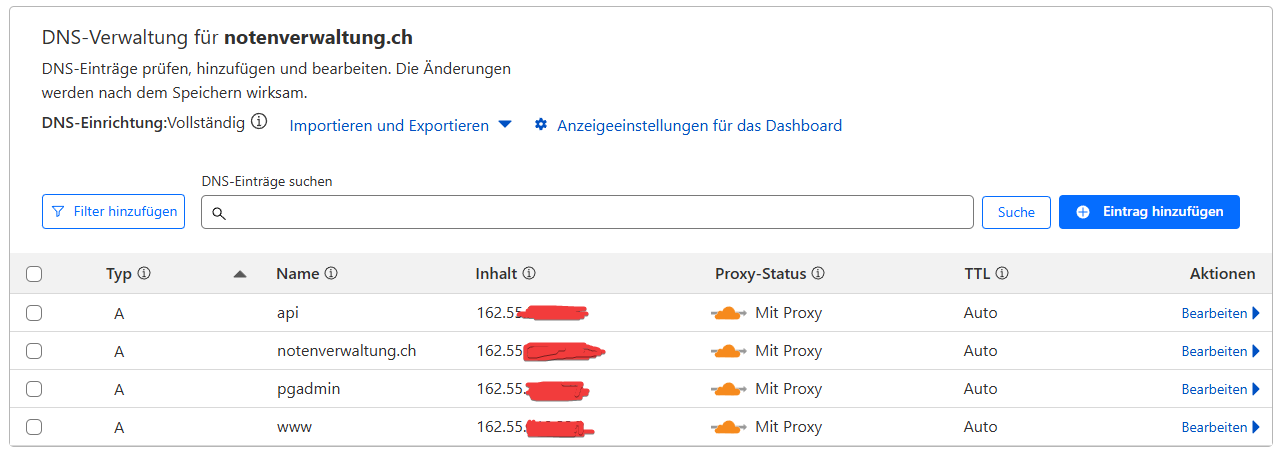
\includegraphics[width=0.95\linewidth]{images/dns}
        \caption{DNS Records in Cloudflare}
        \label{fig:dns}
    \end{figure}

    \subsection{Docker}

    \subsubsection{Installation}
    Docker wird mit den folgenden Befehlen installiert:
    \begin{lstlisting}{language=bash}
# Add Docker's official GPG key:
sudo apt-get update
sudo apt-get install ca-certificates curl
sudo install -m 0755 -d /etc/apt/keyrings
sudo curl -fsSL https://download.docker.com/linux/ubuntu/gpg -o /etc/apt/keyrings/docker.asc
sudo chmod a+r /etc/apt/keyrings/docker.asc

# Add the repository to Apt sources:
echo \
  "deb [arch=$(dpkg --print-architecture) signed-by=/etc/apt/keyrings/docker.asc] https://download.docker.com/linux/ubuntu \
  $(. /etc/os-release && echo "${UBUNTU_CODENAME:-$VERSION_CODENAME}") stable" | \
  sudo tee /etc/apt/sources.list.d/docker.list > /dev/null
sudo apt-get update
        
sudo apt-get install docker-ce docker-ce-cli containerd.io docker-buildx-plugin docker-compose-plugin
sudo apt-get install docker-compose
    \end{lstlisting}
    Basierend auf der offiziellen Anleitung von Docker\cite{docker-ubuntu-install}.


    \subsection{Container}
    Damit die Container miteinander kommunizieren können, wird ein Docker Netzwerk erstellt.
    \subsubsection{Docker Netzwerk Anlegen}
    \begin{lstlisting}{language=bash}
    docker network create notenverwaltung_productive
    \end{lstlisting}


    \subsubsection{HTTPs}
    Für die HTTPS Verschlüsselung wird mit hilfe von Cloudflare ein kostenloses SSL Zertifikat erstellt.
    Dieses wird in der NGINX Konfiguration eingebunden.



    \subsubsection{Reverse Proxy}

    todo stack yml

    \subsubsection{Datenbank \& PG Admin}

    todo stack yml

    needed to change permissions


    \begin{lstlisting}{language=bash}
        sudo mkdir -p /mnt/volume-nbg1-1/data/db/pgadmin
        sudo chown -R 5050:5050 /mnt/volume-nbg1-1/data/db/pgadmin
        sudo chmod -R u+rwX /mnt/volume-nbg1-1/data/db/pgadmin
    \end{lstlisting}

    todo pgadmin.conf datei

    \subsubsection{Notenverwaltung Applikation}

    \subsubsection{Angular Frontend + Webserver}


    \section{Verwendung}


    \section*{Quellen}
    \begin{thebibliography}{9}
        \bibitem{docker-ubuntu-install}
        Docker, Inc. "Install Docker Engine on Ubuntu — Install using the repository." Zugriff am 20.09.2025. Verfügbar unter: \url{https://docs.docker.com/engine/install/ubuntu/#install-using-the-repository}
    \end{thebibliography}

\end{document}